%%%%%%%%%%%%%%%%%%%%%%%%%%%%%%%%%%%%%%%%%%%%%%%%%%%%%%%%%%%%%%%%%%%%%%%%%%%%%%%%
% Template for USENIX papers.
%
% History:
%
% - TEMPLATE for USENIX papers, specifically to meet requirements of
%   USENIX '05. originally a template for producing IEEE-format
%   articles using LaTeX. written by Matthew Ward, CS Department,
%   Worcester Polytechnic Institute. adapted by David Beazley for his
%   excellent SWIG paper in Proceedings, Tcl 96. turned into a
%   smartass generic template by De Clarke, with thanks to both the
%   above pioneers. Use at your own risk. Complaints to /dev/null.
%   Make it two column with no page numbering, default is 10 point.
%
% - Munged by Fred Douglis <douglis@research.att.com> 10/97 to
%   separate the .sty file from the LaTeX source template, so that
%   people can more easily include the .sty file into an existing
%   document. Also changed to more closely follow the style guidelines
%   as represented by the Word sample file.
%
% - Note that since 2010, USENIX does not require endnotes. If you
%   want foot of page notes, don't include the endnotes package in the
%   usepackage command, below.
% - This version uses the latex2e styles, not the very ancient 2.09
%   stuff.
%
% - Updated July 2018: Text block size changed from 6.5" to 7"
%
% - Updated Dec 2018 for ATC'19:
%
%   * Revised text to pass HotCRP's auto-formatting check, with
%     hotcrp.settings.submission_form.body_font_size=10pt, and
%     hotcrp.settings.submission_form.line_height=12pt
%
%   * Switched from \endnote-s to \footnote-s to match Usenix's policy.
%
%   * \section* => \begin{abstract} ... \end{abstract}
%
%   * Make template self-contained in terms of bibtex entries, to allow
%     this file to be compiled. (And changing refs style to 'plain'.)
%
%   * Make template self-contained in terms of figures, to
%     allow this file to be compiled. 
%
%   * Added packages for hyperref, embedding fonts, and improving
%     appearance.
%   
%   * Removed outdated text.
%
%%%%%%%%%%%%%%%%%%%%%%%%%%%%%%%%%%%%%%%%%%%%%%%%%%%%%%%%%%%%%%%%%%%%%%%%%%%%%%%%

\documentclass[letterpaper,twocolumn,10pt]{article}
\usepackage{styles}

% to be able to draw some self-contained figs
\usepackage{tikz}
\usepackage{amsmath}

% inlined bib file
\usepackage{filecontents}

%-------------------------------------------------------------------------------
\begin{filecontents}{\jobname.bib}
%-------------------------------------------------------------------------------
@Book{arpachiDusseau18:osbook,
  author =       {Arpaci-Dusseau, Remzi H. and Arpaci-Dusseau Andrea C.},
  title =        {Operating Systems: Three Easy Pieces},
  publisher =    {Arpaci-Dusseau Books, LLC},
  year =         2015,
  edition =      {1.00},
  note =         {\url{http://pages.cs.wisc.edu/~remzi/OSTEP/}}
}
@InProceedings{waldspurger02,
  author =       {Waldspurger, Carl A.},
  title =        {Memory resource management in {VMware ESX} server},
  booktitle =    {USENIX Symposium on Operating System Design and
                  Implementation (OSDI)},
  year =         2002,
  pages =        {181--194},
  note =         {\url{https://www.usenix.org/legacy/event/osdi02/tech/waldspurger/waldspurger.pdf}}}
\end{filecontents}

%-------------------------------------------------------------------------------
\begin{document}
%-------------------------------------------------------------------------------

%don't want date printed
\date{}

% make title bold and 14 pt. font (Latex default is non-bold, 16 pt.)
\title{\Large \bf Evaluation of D v.2.096 for Secure Camera-based HVAC Control}

\maketitle

%-------------------------------------------------------------------------------
\begin{abstract}
%-------------------------------------------------------------------------------
This research was conducted in order to determine if D is viable for 
acting as a replacement for a camera-based HVAC system written in C/C++. Through
thorough analysis of D's documentation and source code examples, pros and cons
of D were evaluated and applied to the requirements of this system and its
users. In the end it was determined that D is not a good fit for replacing C/C++
in this situation, and it would be better if a more suitable language was used
instead.

\end{abstract}

%-------------------------------------------------------------------------------
\section{Introduction}
%-------------------------------------------------------------------------------
\par
A HEAT system uses inexpensive cameras to implement facial temperature detection
software, allowing for precise room temperature adjustments. The company
Haversack Inc., which designs such systems is having trouble marketing these
systems, which are currently written in C and C++. The low-level nature of these
languages makes systems written in them vulnerable to attacks that may
compromise the security of Haversack Inc.'s clients. However, languages such as
Java or Python have bloated frameworks that may also make room for security
vulnerabilities. As an alternative to these, a detailed investigation of D
will be committed in order top determine its effectiveness at implementing the
desired software.

%-------------------------------------------------------------------------------
\section{Strengths and Weaknesses}
%-------------------------------------------------------------------------------
This analysis will focus on the characteristics of the D language itself,
without consideration of the application goals or any external factors. 

\subsection{Security and Reliability}
Typically, D programming tends to fall within the realm of the SafeD
subset of D. Unlike C, code written in SafeD offers protections against
undefined behavior. It does so by relying on the generation of additional 
compile-time checks using templates and the use of tuples to manage parameters.
All this additional static time checking helps programmers avoid potential
undefined behavior in their written code, and can help free them from the
security threats that may arise from lower-level's progression.
\par
One part of SafeD is the ability to implement contracts in your code.
These are additional runtime checks that you can write, such that if your
program reaches that point in execution without satisfying the contract, then
it assumes that some undefined behavior must have occurred to throw it off. 
\par
Another useful feature of D is that it automatically initializes variables,
unlike its predecessor C. This allows programs written in D to completely
ignore an entire subset of potential failures at the cost of runtime
performance.
\par
Finally, D comes with built-in exception handling using the
\texttt{try-catch-finally} structure present in Java. This allows programmers to
prepare for potential failures that may occur during runtime before they
actually happen, allowing an aware programmer to avoid even more subsets of
failures.
\par
The largest potential downfall with D's performance is that, much like C, D
doesn't statically check for null references. These can be very common bugs that
appear in programs, and may be hard to recover from. Although it's possible to
catch them with exception handling, the fact that they can exist in the first
place acts as a potential risk for exploitation, as pointers are directly
handled by the programmer rather than working under the hood like in the JVM.

\subsection{Ease of Use}
One of the larger selling points of D is that it takes on a C-like syntax.
This is especially useful, as the system was previously written in C/C++.
\par
Unlike the C language, D does have an option to use its built-in garbage
collector. This makes memory allocation trivial and makes developing and
debugging much easier for a system, as the developer doesn't have to manually
work with any deallocation code. 
\par
Another useful, built-in feature of D is unit testing. Unit tests are a built-
in framework of test cases that are run before the program starts up. This
simplifies the testing process for the developer, allowing for the
standardization and automation of test cases. These can be easily enabled or
disabled by the programmer, allowing for their use during testing, but their
simple disuse during production.
\par
D also allows for the local import of modules, a feature targeted at making code
more readable. This is especially helpful for a collaborative environment, where
it may be challenging for multiple developers working on the same project to
gain a full understanding of the code.
\par
The biggest downside in terms of usability for D may come from the nature of
lower-level languages. These tend to be harder to read, as more complex
operations take many more lines of code to implement than in a higher-level
language like Python. For instance, one by-product of this is attribute creep,
where functions can be decorated with too many attributes that allow programmers
to alter the function's behavior, resulting in less readability, and a greater
need for in-depth knowledge of the language.

\subsection{Flexibility}
D implements generic programming much like C, using templates instead of
generics. This includes the ability to use template constraints for more control
over parameter checking, template mixins to take code from the body of a
template declaration and use it elsewhere, and implicit function template
instantiation, where template arguments can be deduced from the type of its
arguments.

\par
D also provides a way to directly access C functions and APIs, using
\texttt{extern C++, ...}. This allows for D to work hand in hand with the
C code that may already exist and pull on APIs that programmers are more
familiar with.

\subsection{Performance}
One aspect of D that may provide a boost in performance is its ability to
give programmers direct access to memory management. If the programmer is able
to determine a more efficient way of handling memory that the compiler can't
see, they are free to subvert the built-in garbage collector and implement it
more efficiently.
\par
In addition, D supports an inline assembler, which gives the programmer the
ability to handle assembly code, playing to D's existence as a low-level
language. This allows for programmers to have even more control over how their
program executes, allowing them to escape the compiler's optimizations if they
find a more optimal alternative.
\par
By far, the worst aspect of D when it comes to performance is the garbage
collector. Although it's technically possible to write code that avoids the GC,
that requires abandoning many essential language features of D in the first
place. As a result, D programs will generally fall victim to the stop-the-world
nature of D's garbage collector, where all threads are stopped in order for
garbage collection to finish successfully, possibly tanking performance.

%-------------------------------------------------------------------------------
\section{Application-Relevant Analysis}
%-------------------------------------------------------------------------------
\par
This analysis will focus on appropriating the characteristics of D discussed in
the previous section to the implementation of the camera-based HVAC system.

\subsection{Porting}
One big advantage in switching to D over any other language is its ability to
make use of existing C code and APIs. This feature not only gives the
development team an easier time transitioning to D, but it also allows them to
simply reuse their existing code. In terms of development time, this is huge for
them, as they don't have to waste extra time rewriting the same code they've
already developed.

\subsection{Interfacing}
D comes with the ability to interface directly with hardware. This is perfect
for the system's requirement to interface with the cameras or network interface.
This accessing can be done through the program's assembler, meaning it is fast
and efficient, in addition to it being convenient for the programmer.

\subsection{Readability}
Due to the influence of C, D comes off as a generally readable and debuggable
language. This basis works in conjunction with D's built-in unit testing and 
modularity, making any written code easy to maintain and audit when necessary.

\subsection{Garbage Collector}
The largest issue with D's usage comes in the form of the garbage collector.
D doesn't make use of a garbage collector with OS kernel control, but instead
packages it as a module to be imported into the code. This makes way for the
additional vulnerability that using a non-Java/Python language was meant to
avoid. Although it is theoretically possible to write D code without making use
of this garbage collector, it prevents the usage of many aspects of D that rely
on the GC for functionality. In addition, by opting to not use the garbage
collector, the programmer makes the software vulnerable to exploitation through
poorly-managed memory allocation and deallocation, which D may not be tailored
to address.

%-------------------------------------------------------------------------------
\section{Conclusions}
%-------------------------------------------------------------------------------
\par
Overall, although D is advertised as an improvement on C++, it doesn't seem like
it would be a particularly good alternative for this system. D is likely
serviceable in terms of its performance, reliability, and usability. D fails to
introduce any significant benefits to system security apart from protecting
against certain subsets of failures. This protection comes at the cost of an
added garbage collector, which may tank performance while adding extra security
concerns that clients would like to avoid. Although D does provide the option to
operate without the use of the garbage collector, unlike Java and Python, this
decision would likely prevent the use of too many of D's features. Even if the
program could still be written with this smaller subset of D, it would then be
just as vulnerable as C to potential attacks on the low-level nature of its
implementation. As a result, although D does have some advantages over the
current C/C++ implementation, the new problems it introduces make it an unfit
replacement for the system. A different language should be used instead.

%-------------------------------------------------------------------------------
\section{References}
%-------------------------------------------------------------------------------
"Documentation"
Updated March 11, 2021 \\
Available: \\ https://dlang.org/documentation.html \\
\\
"Language Issues"
Updated February 28, 2017 \\
Available: \\ https://wiki.dlang.org/Language\_issues \\
\\
P. Eggert "Homework 6. Evaluate a language for secure camera-based HVAC control" 
Updated March 4, 2021. \\
Available: \\ https://web.cs.ucla.edu/classes/winter21/cs131/hw/hw6.html \\


%%%%%%%%%%%%%%%%%%%%%%%%%%%%%%%%%%%%%%%%%%%%%%%%%%%%%%%%%%%%%%%%%%%%%%%%%%%%%%%%
\end{document}
%%%%%%%%%%%%%%%%%%%%%%%%%%%%%%%%%%%%%%%%%%%%%%%%%%%%%%%%%%%%%%%%%%%%%%%%%%%%%%%%

%%  LocalWords:  endnotes includegraphics fread ptr nobj noindent
%%  LocalWords:  pdflatex acks

% \begin{figure}
%   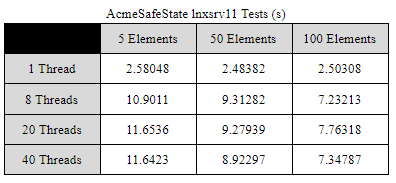
\includegraphics[scale=0.8]{acmesafe-11.png}
%   \caption{\label{fig:vectors} Table of total time results from testing AcmeSafeState on lnxsrv11, measured in seconds. }
% \end{figure}